\documentclass[assignment03_Solutions]{subfiles}

\IfSubStr{\jobname}{\detokenize{Solutions}}{\toggletrue{solutions}}{\togglefalse{solutions}}

\fancypagestyle{firstpage}

{\rhead{Assignment 3 \linebreak \textit{Version: \today}}}

\title{Assignment 3: Probabilistic Definitions of Fairness and Bayesian Networks}
\author{Machine Learning}
\date{Fall 2021}
\invalidatemargin

\begin{document}

\maketitle
\thispagestyle{firstpage}


\begin{learningobjectives}
\bi
\item Learn about the connection between probabilistic criteria for algorithmic fairness and Bayesian Networks.
\item Solidify your understanding of the Na\"ive Bayes algorithm by applying it to movie review sentiment classification.
\ei
\end{learningobjectives}


\section{Reflecting on COMPAS and Algorithmic Fairness}

In assignment 1 of this module we discussed how Bayesian methods can be used to reason about algorithmic fairness.  In class, we discussed fairness within the context of the COMPAS algorithm and the United States justice system.


\begin{exercise}[(15 minutes)]
Please reflect on the conversation in class about the COMPAS algorithm, the US justice system, race in the US, and algorithms and fairness. You can reflect on these topics and/or on the conversation itself (meta). We look forward to hearing your thoughts and appreciate any ideas you have to improve these types of conversations in the future. We are all learning together.\\

Additionally, if you would like to share something anonymously, here is an \href{https://docs.google.com/forms/d/e/1FAIpQLSf1NUDOQR6I0PcNyuaitbShR38pq5AgAiZnFnHtJCa28O-F4Q/viewform?usp=sf_link}{anonymous survey}.

\end{exercise}


\section{Measures of Bias}
In the last assignment, we looked at confusion matrices and different metrics that can be calculated for a single confusion matrix. Now, we will look at some metrics for comparing two confusion matrices (e.g., if we break our results up to look at the outcomes for two different groups).\\

As we saw in the COMPAS debate, confusion matrix metrics are often used to measure fairness and bias. Note that when we say algorithmic bias and fairness, we are referring to the phenomenon of models discriminating against protected or underprivileged groups (based on attributes such as race and gender), which often arises as a factor of bias that is integrated into the dataset used for training. This is common, because datasets often measure phenomena that are already subject to systemic bias and may include additional (usually unintended) bias introduced by the collectors and analysts of the data.\\ 
When detecting algorithmic bias, we typically identify a protected class (such as people of color or women). Many of the popular measures of bias compare the confusion matrix metrics we went over in the last section between the protected and privileged class, either by taking a straightforward difference, or by taking a ratio between the values of the two metrics. These are often referred to as parity of a given metric, for example False Positive Rate Parity, which measures the difference in False Positives of the two groups. Many of the most commonly used metrics have a second name, for example the Equal Opportunity Difference is the same as True Positive Rate Parity.\\
There are many measures of bias, but today we will be focusing on the five common metrics. By understanding these metrics, you will have the tools to understand other, similar metrics that you may want to use in the future. It may be helpful to refer to the \href{http://research.google.com/bigpicture/attacking-discrimination-in-ml/}{loan example visualization from Google Research} again to wrap your head around this.
\begin{itemize}
    \item \textbf{Statistical Parity Difference} is computed as the difference of the rate of favorable outcomes received by the unprivileged group to the privileged group. (Statistical parity is also called Independence or Demographic Parity.)
    \begin{itemize}
        \item The ideal value of this metric is 0.
        \item Fairness for this metric is between -0.1 and 0.1.
        \item Calculated as the difference between predicted positive of the privileged and unprivileged groups.
        \item A value of < 0 implies higher benefit for the privileged group and a value > 0 implies higher benefit for the unprivileged group.
    \end{itemize}
    \item \textbf{Equal Opportunity Difference} is computed as the difference of true positive rates between the unprivileged and the privileged groups.
    \begin{itemize}
        \item The ideal value of this metric is 0.
        \item A value of < 0 implies higher benefit for the privileged group and a value > 0 implies higher benefit for the unprivileged group.
        \item Fairness for this metric is between -0.1 and 0.1
        \item Calculated as the difference between the privileged TPR and unprivileged TPR.
    \end{itemize}
    \item \textbf{Average Odds Difference} is computed as the average difference of false positive rate and true positive rate between unprivileged and privileged groups.
    \begin{itemize}
        \item The ideal value of this metric is 0.
        \item A value of < 0 implies higher benefit for the privileged group and a value > 0 implies higher benefit for the unprivileged group.
        \item Fairness for this metric is between -0.1 and 0.1
        \item Calculated as the average of the difference between the privileged FPR and unprivileged FPR and the difference between the unprivileged TPR and privileged TPR
    \end{itemize}
    \item \textbf{Disparate Impact} is computed as the ratio between rate of favorable outcomes for the unprivileged group to that of the privileged group.
    \begin{itemize}
        \item The ideal value of this metric is 1.0.
        \item A value < 1 implies higher benefit for the privileged group and a value >1 implies a higher benefit for the unprivileged group.
        \item Fairness for this metric is between 0.8 and 1.2.
        \item Calculated as unprivileged predicted positive/privileged predicted positive.
    \end{itemize}
    \item \textbf{Theil Index} is computed as the generalized entropy of benefit for all individuals in the dataset, with alpha = 1. It measures the inequality in benefit allocation for individuals. This is a measure of non-randomness or redundancy.
    \begin{itemize}
        \item A value of 0 implies perfect fairness.
        \item Fairness is indicated by lower scores, higher scores are problematic.
        \item We will not focus on this metric, but \href{https://en.wikipedia.org/wiki/Theil_index}{Wikipedia has a decent article about it.}
    \end{itemize}
\end{itemize}

Sometimes these metrics conflict, so we need to choose carefully based on our application which ones to minimize. 

\begin{exercise}[(60 Minutes)]
\bes
\item Calculate the Statistical Parity Difference, Equal Opportunity Difference, Average Odds Difference, and Disparate Impact of the confusion matrices below. What do you notice? Is this model fair?

%\begin{center}
%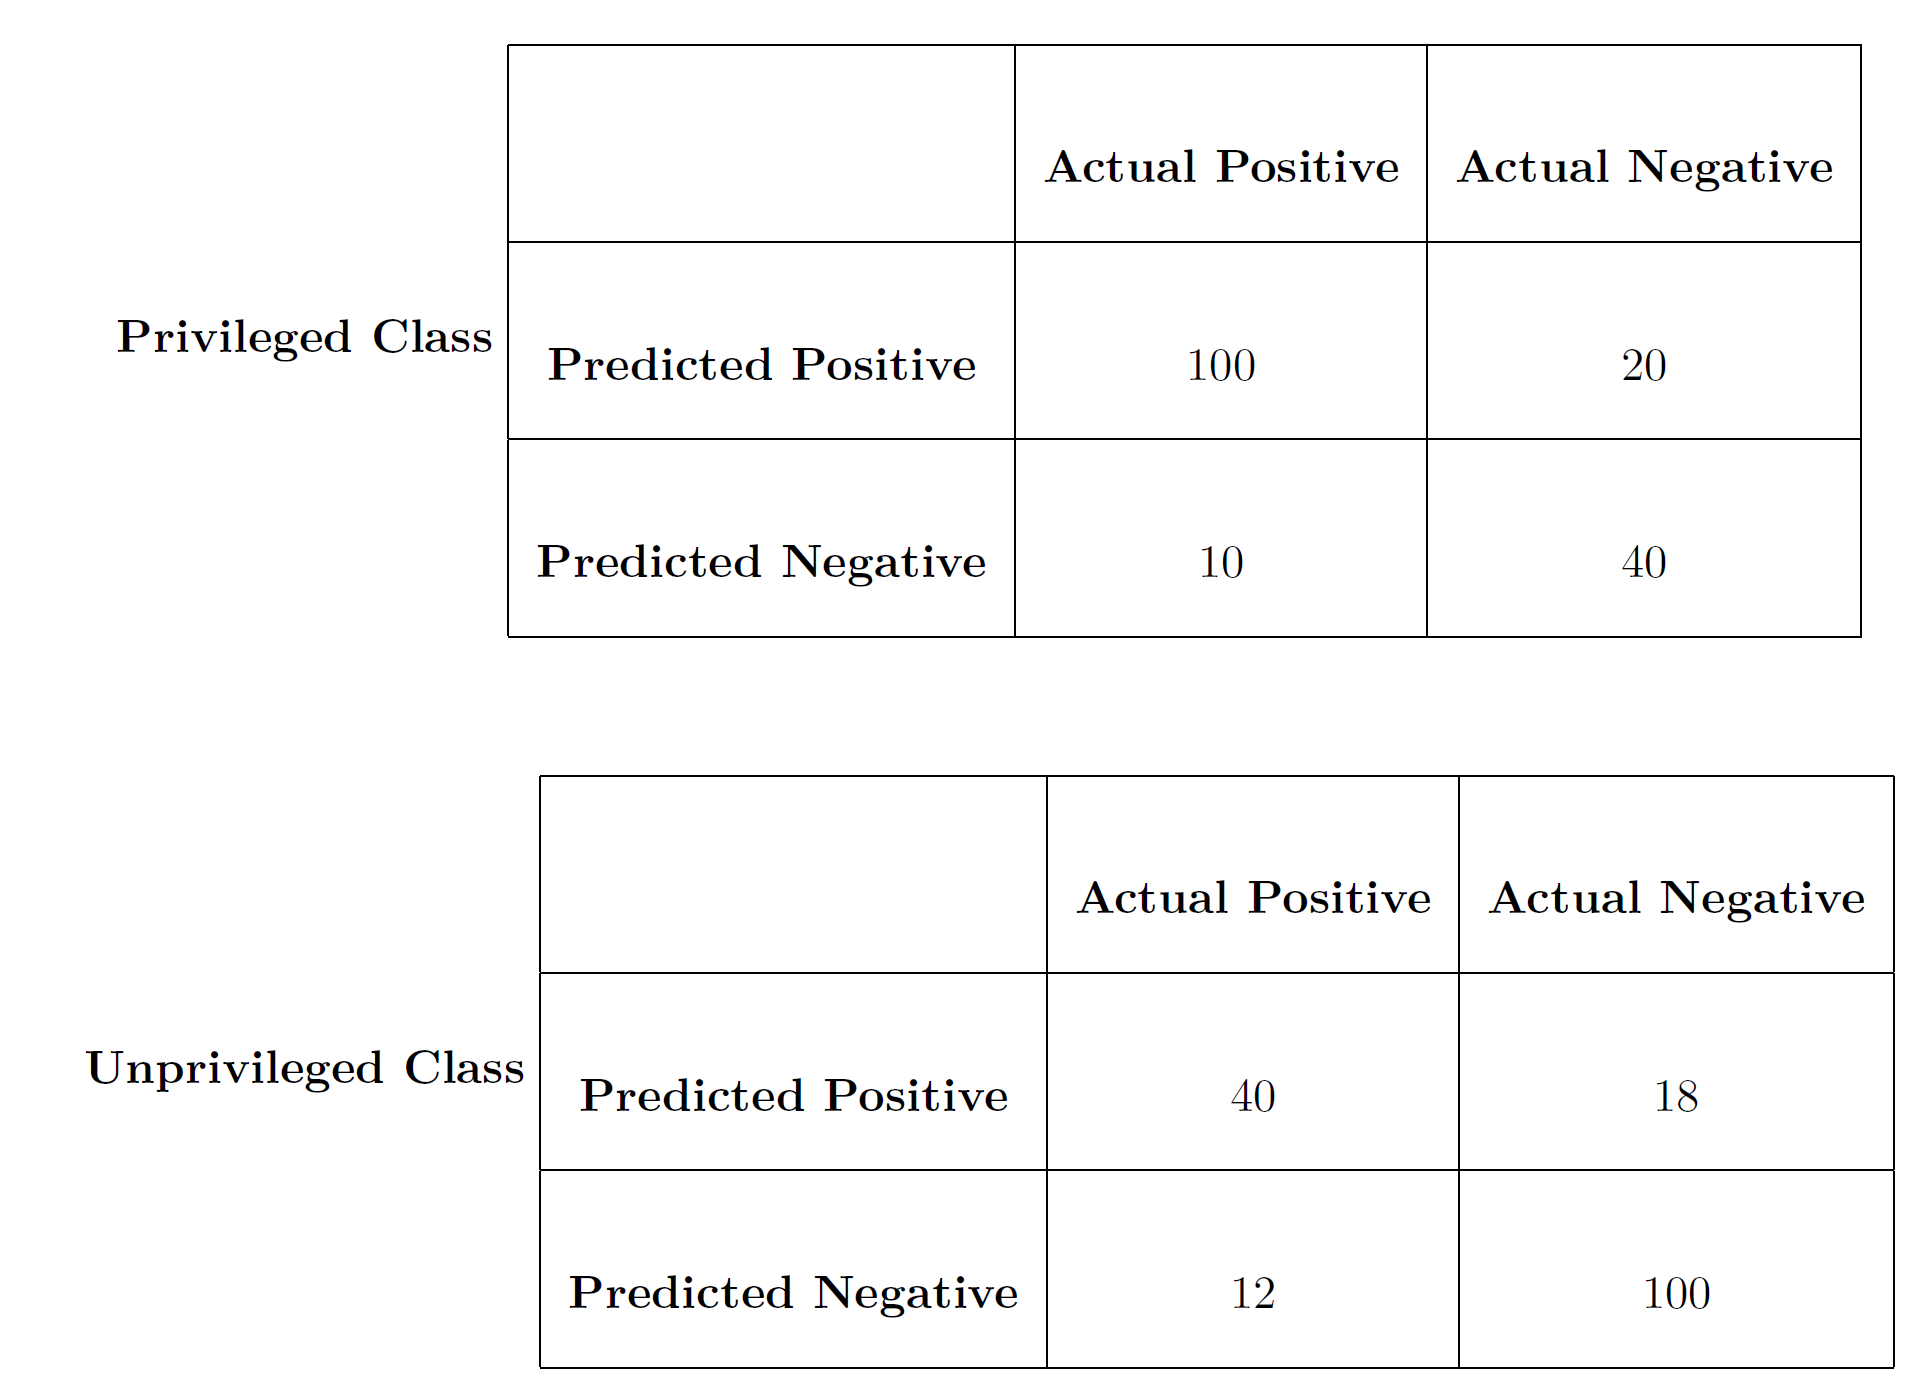
\includegraphics[width=0.5\linewidth]{figures/confusionPrivUnpriv}
%\end{center}


\begin{boxedsolution}
\textbf{Statistical Parity Difference}\\
= (TP + FP)/(total population) of privileged group - (TP + FP)/(total population) of unprivileged group\\
=  (40 + 18)/(40 + 18 + 12 + 100) - (100 + 20)/(100 + 20 + 10 + 40)\\
= 58/170 - 120/170\\
$\approx -0.36$\\
By this metric, the model is quite unfairly biased against the unprivileged group.\\
\textbf{Equal Opportunity Difference}\\
= TP/(TP + FN) of unprivileged group - TP/(TP + FN) of privileged group\\
= 40/52 - 100/110\\
$\approx -0.14$\\
This is close to the window of fairness, but there is still bias against the unprivileged group.\\
\textbf{Average Odds Difference}\\
= (unprivileged TPR - privileged TPR)/2 + (privileged FPR - unprivileged FPR)/2\\
= (TP/(TP + FN) of unprivileged group - TP/(TP + FN) of privileged group)/2 + (FP/(FP + TN) of privileged group - FP/(FP + TN) of privileged group)/2\\
= -.14/2 + (20/60 - 18/100)/2\\
$\approx 0.007$\\
By this definition the model is fair, since the privileged class has a worse False Positive Rate which cancels out the fact that the unprivileged class has a worse True Positive Rate.\\
\textbf{Disparate Impact}\\
= ((TP + FP)/total population of unprivileged group)/((TP + FP)/total population of privileged group)\\
=(58/170)/(120/170)\\
$\approx .48$\\
By this metric, our model is strongly biased against our unprivileged group.\\
As we can see, it is good to check a variety of metrics, because sometimes a model can be strongly biased by most metrics, but still fall within the window of fairness for one or two metrics.
\end{boxedsolution}

\item The Data Science and Public Policy group at Carnegie Mellon University created a decision tree with proposed guidance about which metrics of fairness might be desirable in different situations. Take a look at  \href{http://www.datasciencepublicpolicy.org/wp-content/uploads/2018/05/metrictree-1024x640.png}{their decision tree}. Try to understand why each decision leads to the metrics that it does. 

\ees
\end{exercise}



\section*{The Impossibility Theorem of Fairness}
As we explored in the previous problems, we often cannot satisfy every fairness metric at the same time. This leads to an interesting ethical discussion about when it is appropriate to use a given metric, and when it is okay to accept a failing score on a given fairness metric. Above we show a decision tree for certain metrics that we took from \href{http://www.datasciencepublicpolicy.org/our-work/tools-guides/aequitas/}{Aequitas}, a bias detection toolkit created by the University of Chicago Center for Data Science and Public Policy (now at Carnegie Mellon). 
 
Choosing a fairness metric in a way that is ethical is a highly subjective task. Even though decision trees exist to help policymakers and model creators evaluate their models, this is an active area of research and discussion. One great resource for learning about up and coming developments in this field is \href{https://facctconference.org/}{the FAccT conference}, where researchers and technologists discuss and present research on Fairness, Accountability, and Transparency in ML. At the heart of these debates is the Impossibility Theorem of Fairness, which essentially says that there are many fairness metrics that are mutually exclusive in the vast majority of cases. 

\begin{externalresources}[60 Minutes]
\href{https://www.youtube.com/watch?v=jIXIuYdnyyk}{This lecture on the tradeoffs of different fairness metrics} talks about the societal impact of different fairness metrics, and explains the Impossibility Theorem of Fairness in more depth.
\end{externalresources}

\begin{understandingcheck}
What is group fairness? What is individual fairness? Why are these two notions of fairness in conflict?
\begin{boxedsolution}
Group fairness is focused on comparing metrics between privileged and unprivileged groups to ensure that they have comparable outcomes. Individual fairness is focused on treating the same data and situations the same way across individuals regardless of group affiliation. These can be in conflict because often times to achieve equal representation of positive outcomes between groups, the each group needs to have different criteria for triggering a positive outcome, under the assumption that their average input data or situations are not the same.
\end{boxedsolution}

\end{understandingcheck}
\section*{Bias Mitigation}

Now that we have discussed different ways to detect bias, we want to briefly think about how we can reduce bias and algorithmic discrimination. There are various toolboxes that have been designed to help mitigate bias in algorithms and data, including \href{http://www.datasciencepublicpolicy.org/our-work/tools-guides/aequitas/}{Aequitas (from Carnegie Mellon - this also includes a more detailed decision tree)} and the \href{http://aif360.mybluemix.net/data}{IBM AI Fairness 360 (which you can see a demo of here)}. There are a number of bias mitigation strategies, and each has several variations, but all bias mitigation strategies can be broken up into three categories.
 \subsection*{Pre-processing}
 Pre-processing is the practice of modifying a dataset before training a model. Models learn bias from uneven representation in datasets, stemming from problems with sampling distribution, or from existing social phenomena that create uneven distribution of input situations and outcomes between demographic groups. The theory behind preprocessing is that if a dataset represents a fair distribution of outcomes between demographic groups, any model trained on that data will learn to classify in a fair manner. Preprocessing is often the preferred method of bias mitigation, since it allows for transparency in the bias mitigation process, and it does not change the model training process. It also allows for those who release datasets to ensure that models using those datasets are fair, regardless of who is making them. However, it requires foresight to use since it needs to be implemented before the model is trained, so often model creators opt for in-processing or post-processing.
 \subsection*{In-processing}
 In-processing is the practice of considering notions of fairness while training a model. This is often done by integrating fairness metrics into the error or optimization function while training. In-processing is popular because it builds fairness directly into the model design, unlike pre-processing that only builds fairness into the training data.
\subsection*{Post-processing}
Post processing is the practice of modifying an existing model’s output to satisfy notions of fairness. Post-processing only focuses on group fairness, and it does not consider individual fairness. For this reason, post-processing is often less preferable that the other types of bias mitigation algorithms, which have to ability to consider both group fairness and individual fairness. However, post-processing is a good choice when a model is already trained and cannot be rebuilt.




%\section{Bayesian Networks and Algorithmic Fairness}
%
%
% We touched upon some of the limitations of statistically based notions of fairness.  Nevertheless, these criteria do have a potential role to play, and you should know what the most common definitions of fairness are and what assumptions they make.
%
%As context for the reading and to help us have common notation, suppose we have the following random variables.
%
%\bi
%\item $R$ represents the prediction generated by our algorithm.
%\item $A$ represents a sensitive attribute
%\item $Y$ represents the thing we're trying to predict (we want $R = Y$ if we are accurate)
%\ei
%
%
%\begin{externalresources}[(40 minutes)]
%Read \href{https://fairmlbook.org/classification.html}{Fairness and Machine Learning Chapter 2}.  Start at the section \emph{Formal non-discrimination criteria} and read up to (but not including) the section \emph{Calibration and sufficiency}.
%\begin{notice}
%\bi
%\item Don't get too hung up on the \href{https://en.wikipedia.org/wiki/Receiver_operating_characteristic}{ROC curves}.  We can discuss this on NB, but it is not required to understand what is going on here.  If you decide to check it out, you'll see an example of an ROC curve in the notebook linked below (it is optional).
%\item The notation they use in this reading for conditional independence is $\bot$ (instead of our notation, $\condindep$).
%\ei
%\end{notice}
%\end{externalresources}
%
%
%\begin{exercise}[(10 minutes)]
%Thinking back to the COMPAS example, which definition of fairness given in the reading was ProPublica using?  Which definition of fairness was Northpointe using?
%
%\begin{boxedsolution}
%\bi
%\item Northpointe is using sufficiency $Y \condindep A~|~R$.  You'll notice that in the reading they say that sufficiency is the same thing as matching positive and negative predictive value for all values of the protected attribute.
%\item Propublica is using separation $R \condindep A~|~Y$.  This fairness principle requires the false positive and true positive rates to be the same across for all values of the protected attribute.
%\ei
%\end{boxedsolution}
%\end{exercise}

%If you're interested in examining the Broward County COMPAS data yourself, we have put together \href{https://colab.research.google.com/github/mlfa19/assignments/blob/master/Module\%202/03/Exploring_COMPAS_Data.ipynb}{a notebook that reproduces the calculations that are at the heart of the two competing notions of fairness}.  The notebook is written in with some notebook exercises, but these are totally optional.  We expect that the default will be that folks will just take a look if they want to (or skip this if they don't). If you want to spend some extra time and solidify your understanding of true positive rate, false positive rate, positive predictive value, etc., then it might be worth doing it as a set of exercises.


\section{Generative versus Discriminative Models (5 minutes)}
So far, we have built up some machinery that allows us to work with probabilities.  Next we're going to take this machinery and turn back towards machine learning.  Specifically, we'll be looking at the classification problem and using probability theory to see it in a whole new light.

\href{https://www.youtube.com/watch?v=HHNESCbZqUg}{This short video} provides a quick overview of generative versus discriminative models, which may be helpful prep for reading the next sections.


\subsection{Discriminative Models: a Look Back at Logistic Regression (10 minute read)}

Let's think back to the logistic regression model for binary classification that we learned about in module 1.  Given an input point $\mathbf{x_i}$, the logistic regression algorithm applied a weight vector $\mathbf{w}$ to compute the probability that the corresponding output $y_i$ was 1 via the formula $\sigma(\mathbf{w}^\top \mathbf{x_i}) = \frac{1}{1+e^{-\mathbf{w}^\top \mathbf{x_i}}}$ (recall that $\sigma$ is known as the sigmoid function and serves to squash its input into a number between 0 and 1, which can serve as a valid probability).  While we didn't quite have the vocabulary for it then, what we were really doing was computing a conditional probability.  We can think of $Y_i$ as a random variable that represents the output corresponding to the input $\mathbf{x_i}$ (in the case of binary classification $Y_i$ is either 0 or 1).  We can also think of the input as a random variable $X_i$ (thinking of the input as a random variable will be helpful later in this section).  Framed in this way the logistic regression algorithm computes the following conditional probability:
\begin{align}
p(Y_i = 1 | X_i = \mathbf{x_i}) &= \sigma(\mathbf{w}^\top \mathbf{x_i}) \enspace .
\end{align}

We defined a loss function to specify which weights were better or worse given a training set $(\mathbf{x_1}, y_1), (\mathbf{x_2}, y_2), \ldots, (\mathbf{x_n}, y_n)$.  The details of how we did this are not important to the point we are trying to make now, so it'll suffice to say that learning in a logistic regression model meant tuning the conditional distribution of the outputs (the $Y_i$'s) given the inputs ($\mathbf{x_i}$'s) to fit the training data the best.  This type of model is what is known as a \emph{discriminative model} (the \href{https://en.wikipedia.org/wiki/Discriminative_model}{Wikipedia article on discriminative models} has more details if you are interested).

\vspace{1em}

\begin{understandingcheck}
Intuitively, why does being able to accurately estimate $p(Y = 1 | X = \mathbf{x})$ allow you to classify unseen test data?

\begin{boxedsolution}
In a classification problem we are interested in predicting the output for a given input, $\mathbf{x}$.  If we can accurately calculate $p(Y=1|X = \mathbf{x})$, then we can simply threshold this value at $0.5$ (or whatever makes sense given our application) and predict $Y = 1$ if this condition is met and $Y = 0$ otherwise.
\end{boxedsolution}
\end{understandingcheck}

\subsection{Generative Models (10 minute read)}
The approach outlined above is great, but it's not the only way to approach binary classification (and supervised learning in general).  Since we are interested in predicting $Y_i$ given some inputs $\mathbf{x_i}$, it of course makes sense, for example for a binary classification problem, to want to determine $p(Y_i = 1 | \mathbf{x_i})$.  However, instead of modeling that distribution directly, we can use Bayes' rule.

\begin{align}
p(Y_i  = 1 | X_i = \mathbf{x_i}) &= \frac{p(X_i = \mathbf{x_i} | Y_i = 1) p(Y_i = 1)}{p(X_i = \mathbf{x_i})} \label{eq:pgm} \\
&= \frac{p(X_i = \mathbf{x_i} | Y_i = 1) p(Y_i = 1)}{p(X_i =  \mathbf{x_i} | Y_i = 1) p(Y_i = 1) + p(X_i = \mathbf{x_i} | Y_i = 0) p(Y_i = 0)} \nonumber
\end{align}

These equations tell us is that if we have a model of the probability of the output being 1 \emph{a priori}, $p(Y_i = 1)$, and a model of the inputs $\mathbf{x_i}$ given the output $y_i$, $p(X_i = \mathbf{x_i} | Y_i = y_i)$, then we can compute $p(Y_i = 1 | X_i = \mathbf{x}_i)$.  This amounts to adopting the perspective that the hidden output $Y_i$ causes the input $X_i$.  We call this sort of model a \href{https://en.wikipedia.org/wiki/Generative_model}{probabilistic generative model} (PGM).  The BN corresponding to this model is given below.

\begin{center}
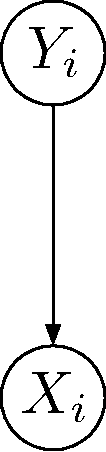
\includegraphics[width=0.05\linewidth]{figures/pgm}
\end{center}


The natural question is \emph{why?} Here are some potential advantages of using probabilistic generative models.
\bi
\item Suppose you found out that $p(Y_i)$ changed for some reason (any thoughts on when this might happen?  Post here on NB).  Incorporating this change into a probabilistic graphical model would be very straightforward (just modify $p(Y_i =1)$ in Equation~\ref{eq:pgm}).
\item Suppose you found out that $p(X_i  = \mathbf{x_i} | Y_i = y_i)$ changed for some reason.  For example, if one of the elements of $X_i$ represents a result obtained by running some sort of medical test, the sensitivity of that medical test might change (any other examples on when this might happen? Post here on NB.).
\item Suppose that instead of classifying data (i.e., predicting $Y_i$), you instead wanted to generate samples $\mathbf{x_i}$ conditioned on a particular value of $Y_i$ (e.g., you might want to \href{https://www.youtube.com/watch?v=LzE1fF0_3q0}{synthesize samples of hand written digits} based on training a probabilistic graphical model).  This can be done naturally with a PGM.  More modern versions of this idea are generative adversarial networks (GANs), which are behind such work as this \href{https://thispersondoesnotexist.com/}{person does not exist} and \href{https://openai.com/blog/better-language-models/}{better language models and their implications} (the second link is the work of a former Oliner!).
\ei

\begin{understandingcheck}
What are the probabilities needed to classify input data in a discriminative model?  What are the probabilities needed to classify input data in a generative model?  How does Bayes' rule connect these two models?

\begin{boxedsolution}
For a discriminative model you need $p(Y=1 | X = \mathbf{X})$.  For a generative model you need $p(Y=1)$ and $p(X = \mathbf{x} | Y=1)$.  Bayes' rule provides the linkage between these two models since one can be transformed into the other simply by applying Bayes' rule.
\end{boxedsolution}
\end{understandingcheck}


\section{Meet the Na\"ive Bayes Algorithm}
Now that we've learned the basic concept of a probabilistic graphical model, let's make things concrete and learn about a specific PGM.  For our first PGM, we're going to learn about the Na\"ive Bayes algorithm (we'll be doing some work with Na\"ive Bayes in the next assignment as well, so you'll have some time to get accustomed to it).  The reason it is called Na\"ive Bayes is that it assumes that all of the observed data ($X_1, X_2, \ldots, X_n$) are conditionally independent given $\mathcal{Y}$.  The BN for the Na\"ive Bayes algorithm is shown below.
\begin{center}
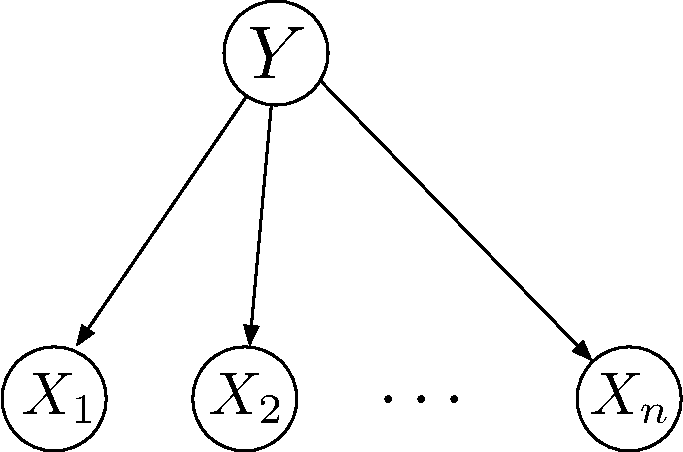
\includegraphics[width=0.3\linewidth]{figures/naivebayesgm}
\end{center}

As a motivating example, let's look back at the Titanic dataset from the last module.  A potential BN for the Titanic dataset is shown below.

\begin{center}
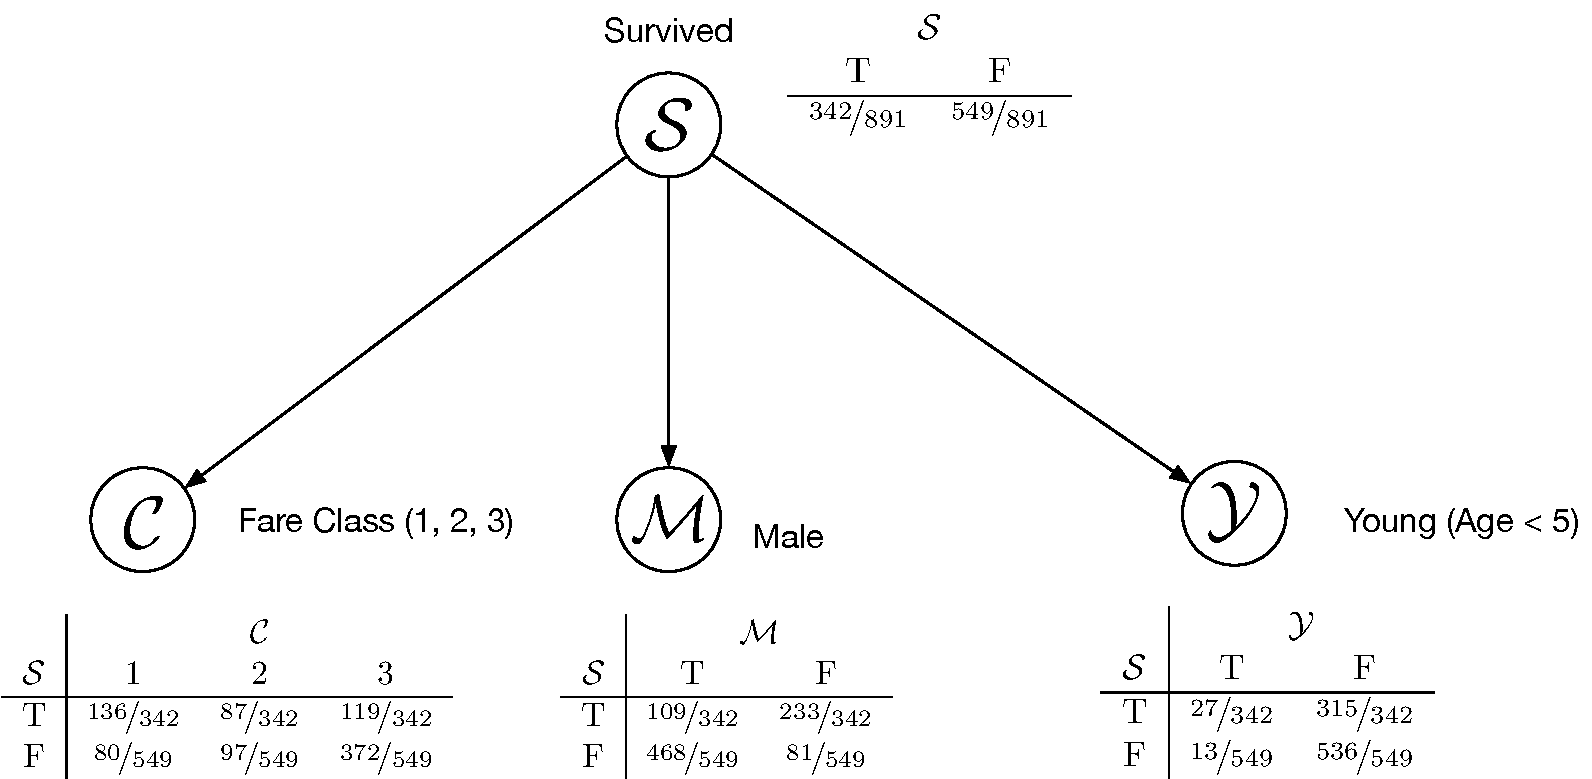
\includegraphics[width=0.8\linewidth]{figures/titanicbn}
\end{center}

The probabilities in this BN were computed by looking at the training set and counting the appropriate passengers that fell into each category.  For instance, to compute $p(\mathcal{Y}|\mathcal{S})$ since $p(\mathcal{Y}|\mathcal{S}) = \frac{p(\mathcal{Y}, \mathcal{S})}{p(\mathcal{S})}$, we can approximate this probability by counting the number of passengers under 5 who survived and dividing by the total number who survived (note that there are some subtle and important modifications to this method of fitting these probabilities that we'll discuss in the next assignment).  This process was repeated for each conditional probability.  Since we assume that all of the features are conditionally independent given the output ($\mathcal{S}$ in this case), this process is done independently for each feature.

\subsection{Inference}
While the Na\"ive Bayes Algorithm might sound fancy, once we have the BN, all we need to do to run the algorithm is to use Bayes' rule.  We'll let you work through this on your own via an exercise.

\begin{exercise}[(45 minutes)]

\bes
\item Using the BN shown above, what is the probability that a young, male in first class would survive the Titanic disaster?  Hint: write this as a conditional probability and then use Bayes' rule.  Hint 2: leverage the fact that $\mathcal{C}, \mathcal{Y}, \mathcal{M}$ are all conditionally independent of each other given $\mathcal{S}$.

You have just derived the Na\"ive Bayes inference rule!

\begin{boxedsolution}
\begin{align}
p(\mathcal{S}|\mathcal{Y}, \mathcal{C}=1, \mathcal{M}) &= \frac{p(\mathcal{Y}, \mathcal{C}=1, \mathcal{M}|\mathcal{S})p(\mathcal{S})}{p(\mathcal{Y}, \mathcal{C}=1, \mathcal{M})} \nonumber \\
&= \frac{p(\mathcal{Y}, \mathcal{C}=1, \mathcal{M}|\mathcal{S})p(\mathcal{S})}{p(\mathcal{Y}, \mathcal{C}=1, \mathcal{M}| \mathcal{S})p(\mathcal{S}) + p(\mathcal{Y}, \mathcal{C}=1, \mathcal{M}|\neg \mathcal{S})p(\neg \mathcal{S})} \nonumber \\
&=  \frac{p(\mathcal{Y}|\mathcal{S}) p( \mathcal{C}=1 | \mathcal{S}) p(\mathcal{M}|\mathcal{S})p(\mathcal{S})}{p(\mathcal{Y}|\mathcal{S}) p( \mathcal{C}=1 | \mathcal{S}) p(\mathcal{M}|\mathcal{S})p(\mathcal{S}) + p(\mathcal{Y}|\neg \mathcal{S}) p( \mathcal{C}=1 | \neg \mathcal{S}) p(\mathcal{M}|\neg \mathcal{S})p(\neg \mathcal{S})} \nonumber \\
&= \frac{\left ( \frac{27}{342} \times \frac{136}{342} \times \frac{109}{342}\times \frac{342}{891}\right)}{\left ( \frac{27}{342} \times \frac{136}{342} \times \frac{109}{342}\times \frac{342}{891} \right ) + \left ( \frac{13}{549} \times \frac{80}{549} \times \frac{468}{549}\times \frac{549}{891} \right )} \nonumber \\
&= 0.6794 \nonumber
\end{align}

\end{boxedsolution}

\item Na\"ive Bayes is often more conveniently expressed using odds ratios.  Instead of computing $p(\mathcal{S}|\mathcal{Y}, \mathcal{C}=1, \mathcal{M})$ let's compute the following.
\begin{align}
\frac{p(\mathcal{S}|\mathcal{Y}, \mathcal{C}=1, \mathcal{M})}{p(\neg \mathcal{S}|\mathcal{Y}, \mathcal{C}=1, \mathcal{M})} &= \frac{\frac{p(\mathcal{Y}, \mathcal{C}=1, \mathcal{M} | \mathcal{S})p(\mathcal{S})}{p(\mathcal{Y},\mathcal{C}=1, \mathcal{M})}}{\frac{p(\mathcal{Y}, \mathcal{C}=1, \mathcal{M} | \neg \mathcal{S})p(\neg \mathcal{S})}{p(\mathcal{Y},\mathcal{C}=1, \mathcal{M})}} \nonumber \\
&=  \frac{p(\mathcal{Y}, \mathcal{C}=1, \mathcal{M} | \mathcal{S})p(\mathcal{S})}{p(\mathcal{Y}, \mathcal{C}=1, \mathcal{M} | \neg \mathcal{S})p(\neg \mathcal{S})} \nonumber \\
&= \frac{p(\mathcal{Y} | \mathcal{S}) p(\mathcal{C}=1 | \mathcal{S}) p(\mathcal{M} | \mathcal{S})p(\mathcal{S})}{p(\mathcal{Y}| \neg \mathcal{S}) p(\mathcal{C}=1 | \neg \mathcal{S}) p(\mathcal{M} | \neg \mathcal{S})p(\neg \mathcal{S})} \nonumber
\end{align}

What must be true about this odds ratio in order to predict that the passenger survived?
\begin{boxedsolution}
The odds ratio must be greater than 1, which implies that
\begin{align}
p(\mathcal{S}|\mathcal{Y}, \mathcal{C}=1, \mathcal{M}) &> p(\neg \mathcal{S}|\mathcal{Y}, \mathcal{C}=1, \mathcal{M}) \enspace . \nonumber
\end{align}
\end{boxedsolution}

\ees
\end{exercise}


\end{document}
